\documentclass[12pt]{report}
\usepackage[utf8]{inputenc}
\usepackage{graphicx}
\usepackage{geometry}
\usepackage{titlesec}
\usepackage[hidelinks]{hyperref}
\renewcommand{\thesection}{\arabic{section}}
\usepackage{hyperref}


% Set the page margins.
\geometry{a4paper, margin=1in}

% Set the section title spacing and format.
\titleformat{\section}
  {\normalfont\Large\bfseries}{\thesection}{1em}{}
\titlespacing*{\section}
  {0pt}{3.5ex plus 1ex minus .2ex}{2.3ex plus .2ex}

% Define custom commands for common elements.
\newcommand{\keyword}[1]{\textbf{#1}}
\newcommand{\characters}[1]{(\textit{min #1 characters})}

% Title Page
\title{EK: Rapor Format}
\author{Your Name}
\date{\today}

% Adjust secnumdepth to ensure sections are numbered
\setcounter{secnumdepth}{3} % Number sections, subsections, and subsubsections

% Adjust tocdepth to control the depth of the ToC
\setcounter{tocdepth}{3} % Include sections, subsections, and subsubsections in the ToC

\begin{document}


% Abstract
\begin{abstract}
The "Crypto Data Analysis and Education Platform" is designed to serve as a comprehensive nexus for learners, investors, and enthusiasts of the cryptocurrency world. This platform stands out by providing real-time market data, educational content, and tools necessary for users to make informed decisions in the fast-paced realm of cryptocurrencies. It aims to demystify the complexities of blockchain technology and crypto assets through a user-friendly interface that caters to both novices and seasoned traders. The educational component is akin to a digital academy, offering courses and materials that range from the fundamentals of blockchain to advanced trading strategies. The analysis feature empowers users with actionable insights into market trends and potential investments. With a focus on security and up-to-date information, the platform integrates various technological solutions, including microservices for scalability, WebSocket for real-time updates, and advanced encryption for data protection. This project stands at the intersection of educational technology and financial innovation, aspiring to enhance the cryptocurrency community's literacy and investment acumen.
\end{abstract}


\textbf{Key Words:} Cryptocurrency Education, Blockchain Technology, Market Analysis, Crypto Portfolio Management, Decentralized Finance (DeFi), Digital Currency Trends, Blockchain Data Visualization, Crypto Trading Strategies, Financial Technology (FinTech), Smart Contract Development, Cryptography and Security, Distributed Ledger Technology, Tokenomics and Cryptoassets, Crypto Exchange Integration, Real-Time Market Data, Crypto Investment Analysis, Blockchain for Education, Crypto Regulatory Compliance, Decentralized Applications (DApps), Cryptocurrency News and Events.


% Add table of contents
\tableofcontents
\renewcommand{\thechapter}{\arabic{chapter}}
\renewcommand{\thesection}{\arabic{section}}
\setcounter{secnumdepth}{3} % Number sections, subsections, and subsubsections
\setcounter{tocdepth}{3} % Include sections, subsections, and subsubsections in the ToC

\newpage

% Introduction
\section{Introduction \characters{5000}}
The rise of blockchain technology and cryptocurrencies has transformed the financial landscape, introducing novel ways of handling transactions and storing value. Pioneered by the innovative designs of Satoshi Nakamoto's Bitcoin and Vitalik Buterin's Ethereum, these technologies provide decentralized solutions that challenge traditional financial and contractual systems \cite{nakamoto2008, buterin2014}.

Blockchain technology, the backbone of cryptocurrencies, operates on a distributed ledger system that enhances transparency and security, reducing the dependency on centralized financial intermediaries. This shift not only revolutionizes how transactions are recorded and verified but also opens up possibilities for automated, trustless contracts known as smart contracts, which Buterin's Ethereum platform popularized.

This platform is designed to bridge the gap between complex blockchain technology and the general public by demystifying crypto concepts and promoting an understanding of its fundamentals through educational resources. Users will have access to a variety of tools that assist in tracking market trends and managing personal crypto portfolios, ensuring they are well-equipped to make informed decisions. Features like real-time market analytics, portfolio risk assessment, and educational webinars are integrated to support both novice and experienced users.

Moreover, the platform will feature real-time updates and analytical insights into the fast-evolving world of cryptocurrencies. By integrating educational content with up-to-date market analysis, the platform seeks to empower users with knowledge and practical tools, making them adept at navigating the crypto market. This real-time data is crucial in a market known for its volatility and rapid changes, providing users with the most current information to base their decisions.

Additionally, the platform will include an extensive range of features such as an admin panel for content management, a blog editor akin to Notion, and an education platform reminiscent of Udemy. These features are designed to enhance user engagement and provide tailored educational experiences, making the platform a central hub for crypto learning and analysis. The inclusion of community-driven content and interactive learning modules further facilitates an engaging learning environment that adapts to the needs of its users.

The societal impact of blockchain extends beyond financial transactions and into areas such as supply chain management, healthcare record keeping, and even voting systems. By reducing fraud, enhancing transparency, and providing unalterable records, blockchain technologies offer significant improvements to critical societal systems.

In essence, the "Crypto Data Analysis and Education Platform" not only serves as a tool for personal portfolio management but also as a beacon of knowledge, contributing to the safety and accessibility of cryptocurrency investments. This project, by addressing the educational gap and providing analytical tools, aligns with the ongoing advancements in cryptocurrency technologies and the increasing global interest in digital currencies. As the landscape of digital currencies continues to evolve, this platform remains committed to providing comprehensive resources and tools to navigate this complex and dynamic field effectively.

As we look to the future, the potential for blockchain to support sustainable and inclusive financial systems becomes increasingly apparent. With ongoing advancements in technology and a growing understanding of its capabilities, blockchain is poised to create significant transformative impacts on global economic and social systems.

Blockchain's ability to automate trust and verify the integrity of transactions without third-party intermediaries fundamentally changes how digital services are provided across industries. This platform takes advantage of blockchain's distributed architecture to ensure that all transactions are transparent and tamper-proof, thereby enhancing user confidence and security. This is especially critical in scenarios involving cross-border transactions, where traditional systems often struggle with trust and efficiency.

The project also addresses potential barriers to adoption, such as the complexity of blockchain technology and the volatility of cryptocurrencies. Through its educational modules, the platform demystifies these barriers and provides a structured pathway for users to gain confidence and understanding in handling digital currencies. Furthermore, we anticipate incorporating adaptive learning technologies that tailor educational content to the user’s progress and understanding, enhancing personalized learning experiences.

Additionally, the environmental impact of blockchain technologies, particularly those reliant on energy-intensive consensus mechanisms like proof of work, is a growing concern. Our platform advocates for the adoption of more sustainable practices within the crypto community and supports the transition towards proof of stake and other less energy-intensive technologies. Educating users about these choices is part of our commitment to promoting sustainability in blockchain development.

Looking forward, the convergence of blockchain with other leading technologies such as artificial intelligence (AI) and the Internet of Things (IoT) promises to further expand its applications. AI can enhance blockchain efficiency by optimizing mining processes and improving security through predictive behavior modeling, while IoT devices can leverage blockchain to secure the vast data they generate. The platform aims to stay at the forefront of these advancements, offering updated content and tools that reflect the latest in technology integration.

As digital currencies and blockchain technologies become more ingrained in everyday business practices, the need for comprehensive and accessible education will continue to grow. The "Crypto Data Analysis and Education Platform" is positioned to be a leader in this space, providing valuable resources that empower individuals and organizations to participate effectively in the digital economy. This initiative not only supports personal investment strategies but also fosters a broader understanding and acceptance of digital currencies as a legitimate component of modern financial systems.

In conclusion, the "Crypto Data Analysis and Education Platform" not only educates and informs but also inspires its users to explore the potential of cryptocurrencies and blockchain technology. By bridging the gap between technological complexity and general understanding, the platform plays a crucial role in shaping the future of finance and technology.

% Realistic Constraints and Conditions
\section{Realistic Constraints and Conditions}

\subsection{Sustainable Development Goal \characters{1000}}
The ``Crypto Data Analysis and Education Platform'' aligns with several United Nations Sustainable Development Goals (SDGs), notably SDG 4: Quality Education, SDG 9: Industry, Innovation and Infrastructure, and SDG 10: Reduced Inequalities. By providing accessible, high-quality educational resources on cryptocurrencies and blockchain technology, the platform contributes directly to SDG 4. It enhances the availability of quality education materials and lifelong learning opportunities for all, regardless of geographic location or economic status.

Innovatively, the platform utilizes cutting-edge technology to disseminate information and provide user-friendly tools for data analysis and portfolio management, aligning with SDG 9. This fosters innovation through the integration of advanced technologies in the educational landscape, promoting a robust infrastructure for learning and engagement in the crypto economy.

Furthermore, by democratizing access to information and financial tools, the platform addresses SDG 10, which aims to reduce inequality within and among countries. It provides equal opportunities for all users to gain financial literacy and participate in the growing digital economy, thereby helping to lessen income and opportunity disparities globally.

Through these contributions, the platform not only advances cryptocurrency education but also plays a pivotal role in promoting sustainable development by integrating educational outreach with technological innovation and inclusivity.

\subsection{Effects on Health, Environment and the Problems of the Age Reflected in the Field of Engineering \characters{1000}}
The ``Crypto Data Analysis and Education Platform'' intersects crucially with contemporary societal and environmental challenges, particularly those addressed in the field of engineering. While cryptocurrencies themselves are often criticized for their environmental impact, primarily due to the energy-intensive nature of mining activities, this platform contributes positively by promoting the adoption of more sustainable blockchain technologies such as proof-of-stake protocols, which require significantly less energy than the traditional proof-of-work systems.

Moreover, the platform encourages the development and use of blockchain applications that can improve public health systems, such as secure and transparent medical record management and supply chain oversight for pharmaceuticals. By integrating advanced data analysis tools, it facilitates more informed decisions that can lead to improved health outcomes and more efficient resource allocation in healthcare settings.

From an engineering perspective, the platform addresses modern problems by promoting technological literacy and accessibility. It provides tools and educational resources that demystify advanced engineering concepts related to blockchain and cryptocurrency technologies, making these topics accessible to a broader audience. This not only helps in reducing the digital divide but also empowers individuals with the knowledge to engage in discussions and activities that shape the future of technology.

Thus, the platform not only enhances understanding and adoption of blockchain technology but also contributes to environmental sustainability and public health through its educational and technological initiatives. These contributions reflect a comprehensive approach to tackling the pressing issues of our time through innovative engineering solutions.

\subsection{Legal Consequences \characters{1000}}
The deployment and operation of the ``Crypto Data Analysis and Education Platform'' entail a thorough navigation of complex legal landscapes, particularly concerning data privacy, cryptocurrency regulations, and intellectual property rights. In the realm of data privacy, adherence to regulations such as the General Data Protection Regulation (GDPR) in Europe and similar laws globally is imperative. The platform is committed to ensuring the confidentiality, integrity, and availability of user data, employing state-of-the-art security measures to protect personal information and transaction details.

Furthermore, as the platform deals with cryptocurrency data and provides tools for financial analysis and management, compliance with financial regulations is crucial. This includes observing the guidelines set by financial authorities regarding the reporting and transparency of cryptocurrency transactions to prevent money laundering and financial fraud. The platform ensures that all features comply with the legal standards of each jurisdiction in which it operates, adapting to ongoing changes in cryptocurrency legislation.

Additionally, the platform must consider intellectual property laws, especially concerning the content generated for educational purposes and the proprietary technology developed for data analysis and portfolio management. This involves securing copyrights for educational content and patents for unique technological innovations, where applicable, to protect the platform’s assets and intellectual contributions.

Navigating these legal requirements is not only necessary for compliance but also crucial in building trust with users and stakeholders. By adhering to these legal standards, the platform ensures its long-term viability and integrity in the highly scrutinized domain of cryptocurrency and blockchain technology.



Here's a comprehensive draft for the "Literature Analysis" section of your report based on a systematic review of the recent literature on cryptocurrency education platforms and blockchain technology's role in education.

\section{Literature Analysis \characters{8000}}
The advent of blockchain technology has sparked a significant interest across various sectors, including education, where it is seen as a potential driver for innovation and trust. A systematic literature review reveals that blockchain technology is increasingly incorporated in educational systems, emphasizing decentralized, secure, and transparent learning environments. This aligns with the objectives of the "Crypto Data Analysis and Education Platform" which seeks to integrate blockchain for educational purposes.

Recent studies highlight blockchain's role in enhancing trust and security in educational transactions, which is crucial for the authenticity of certifications and the management of educational records. Furthermore, the application of blockchain in education extends to facilitating lifelong learning opportunities and supporting decentralized education models. These aspects are particularly pertinent to the platform's goal of providing a comprehensive and trustworthy educational environment on cryptocurrencies and blockchain technology.

Cryptocurrency education platforms also benefit from blockchain's ability to offer transparent and verifiable content, which is essential in an era where the authenticity of educational material can be crucial for both learners and educators. The technology also supports innovative learning solutions that can adapt to the needs of a global audience, fostering a more inclusive educational landscape.

Moreover, the literature identifies a growing trend towards the integration of cryptocurrencies within educational frameworks, either as a subject of study or as a medium for facilitating transactions within educational ecosystems. This dual approach not only enhances understanding of digital currencies but also encourages the practical use of blockchain technology in everyday educational administrative operations.
The integration of blockchain technology in education has been extensively reviewed in the literature, highlighting its transformative potential across various learning environments. Drescher (2017), Mohanty (2021), and Zheng et al. (2018) provide comprehensive analyses of how blockchain technology can be leveraged for educational purposes, discussing its application in certifying student records and creating decentralized educational platforms \cite{drescher2017, mohanty2021, zheng2018}.

Furthermore, the economic and financial implications of blockchain have been critically explored by Tapscott and Tapscott (2016) and Swan (2015). These studies examine how blockchain technology is reshaping financial systems, emphasizing its role in reducing transaction costs and enhancing transparency in financial operations \cite{tapscott2016, swan2015}. Their work underscores the broader impact of blockchain beyond mere cryptocurrency transactions, pointing to a revolution in how global economic infrastructures may evolve.

These scholarly contributions provide a solid foundation for understanding both the educational utility and the economic significance of blockchain technology, highlighting its multidimensional impacts that extend across sectors and disciplines.


The intersection of blockchain technology with educational needs highlights its potential to address several persistent challenges within the sector, including issues of access, verification, and cost-efficiency. By leveraging blockchain, educational platforms can provide more scalable and flexible learning solutions that are aligned with modern technological advancements.

Continuing from the transformative potential of blockchain in educational settings, it is also important to consider the implications for student privacy and data sovereignty. The decentralized nature of blockchain can offer students control over their own educational records, which contrasts sharply with traditional centralized storage systems that are vulnerable to breaches and unauthorized access. By enabling a student-owned data model, blockchain technology empowers individuals with the ability to directly manage and share their academic credentials without intermediaries, enhancing privacy and trust \cite{privacyBlockchain}.

Moreover, blockchain facilitates international educational collaboration by simplifying the validation of credentials across borders. This aspect is particularly advantageous for global educational programs and online learning platforms that attract students from various jurisdictions. Blockchain's ability to seamlessly verify the authenticity of educational records across countries can significantly reduce bureaucracy and enhance the mobility of students and professionals worldwide \cite{internationalBlockchain}.

Additionally, the adoption of blockchain influences educational policies and regulatory frameworks. Educational institutions and policymakers are increasingly recognizing the need to update traditional rules and systems to accommodate and foster the use of blockchain technology. This shift may require new guidelines for interoperability, data sharing, and security standards specific to educational applications of blockchain, promoting a more innovative and adaptive educational landscape \cite{policyBlockchain}.

The use of blockchain in controlling and issuing micro-credentials is another promising area. Micro-credentials offer a way for learners to gain specific, practical skills that are often not covered in traditional education systems. Blockchain's role in securely managing these credentials ensures their credibility and makes them easily shareable with employers or other institutions, thereby enhancing job prospects and lifelong learning paths \cite{microCredentialsBlockchain}.

Moreover, blockchain technology presents unique opportunities for continuous professional development. As workplaces evolve and the demand for new skills accelerates, blockchain platforms can facilitate lifelong learning by providing verifiable and immutable records of learning and professional development activities. This not only benefits individuals seeking to enhance their careers but also employers who require reliable methods to verify the qualifications and ongoing education of their workforce \cite{professionalDevelopmentBlockchain}.

The potential of blockchain to enhance educational accessibility for underserved or remote populations is another critical area of impact. By providing a decentralized platform, blockchain can deliver educational resources with reduced need for robust IT infrastructure typically required by centralized e-learning systems. This can break significant barriers to education in regions where access to quality resources is limited, thereby democratizing education on a global scale \cite{accessibilityBlockchain}.

However, the integration of blockchain technology into education systems is not without challenges. Scalability issues, the energy consumption of certain blockchain models, and the need for substantial initial investment in infrastructure can be significant barriers. Furthermore, ethical considerations regarding student data privacy, the control over educational content, and the potential for unequal access to blockchain-enhanced educational resources must be addressed. These challenges require thoughtful solutions and robust policy frameworks to ensure that the adoption of blockchain technology contributes positively to the educational sector \cite{ethicalBlockchain}.

Lastly, blockchain's role in credentialing extends to the potential for combating academic fraud. The immutable nature of blockchain could significantly reduce incidents of credential falsification, providing a reliable means of verifying academic records and professional certifications. This application not only enhances the integrity of educational and professional credentials but also supports regulatory bodies and employers in maintaining high standards of verification \cite{credentialBlockchain}.

In conclusion, while blockchain technology offers significant benefits to the educational sector, including enhanced trust, improved accessibility, and lifelong learning, it also presents various challenges that need to be navigated carefully. As this technology continues to

\subsection{Features and Requirements of Current Cryptocurrency Education Platforms}
Understanding the features and requirements of existing cryptocurrency education platforms is crucial for designing an effective and user-centric new platform. Köse (2022) provides a detailed analysis of the functionalities that are essential in cryptocurrency education platforms, such as user-friendly interfaces, accessibility features, real-time data processing, and robust security measures \cite{kose2022}. 

Based on Köse's findings, our platform has been designed to include interactive educational tools, comprehensive resource libraries, and integration with real-time market data feeds to ensure that users not only learn about cryptocurrency but also apply their knowledge in real-world scenarios. Additionally, to accommodate users at different levels of expertise, the platform offers customized learning paths that include beginner, intermediate, and advanced courses.

The emphasis on security, as highlighted by Köse, leads us to implement state-of-the-art security protocols, including SSL encryption, two-factor authentication, and regular penetration testing to protect user data and financial information.

By aligning our system's features with the requirements identified in the literature, we aim to provide a superior educational experience that meets the needs of diverse learners interested in cryptocurrencies.


\section{Standards to be Used \characters{1000}}
The ``Crypto Data Analysis and Education Platform'' will adhere to a set of established standards to ensure the reliability, security, and effectiveness of its services. These standards include:

\textbf{ISO/IEC 27001:} This standard is crucial for information security management systems (ISMS), providing a systematic approach to managing sensitive company information so that it remains secure. It includes people, processes, and IT systems by applying a risk management process.

\textbf{WCAG 2.1:} The Web Content Accessibility Guidelines ensure that content is accessible to all users, including those with disabilities. This aligns with the platform's commitment to inclusivity.

\textbf{IEEE Standards:} Utilizing IEEE standards for software development and data interoperability ensures that the platform's technological solutions are robust and adhere to international guidelines for engineering quality.

\textbf{Open Badges 2.0:} For educational achievements, the platform will integrate Open Badges 2.0, a standard to recognize and verify learning achievements with digital badges issued by credible organizations.

\textbf{Cryptocurrency Security Standard (CCSS):} This is essential for ensuring that all systems that use cryptocurrencies adhere to security prerequisites that protect all information within a cryptocurrency system.

These standards are chosen to promote best practices in security, accessibility, education, and data handling, supporting the platform’s mission to provide a trustworthy and inclusive educational environment.

\section{Approaches, Techniques, and Technologies to be used \characters{6000}}
The development and operation of the ``Crypto Data Analysis and Education Platform'' encompass a variety of modern approaches, techniques, and technologies designed to create a robust, scalable, and user-friendly environment. The key aspects include:

\textbf{Microservices Architecture:} Utilizing a microservices architecture, particularly through NestJS, enables the platform to be highly scalable and maintainable. This architecture allows for the independent scaling of different parts of the application, which is essential for handling varying loads and introducing new features without downtime.

\textbf{React Native and Expo for Mobile Development:} These technologies allow for the development of cross-platform mobile applications that provide a native app experience. React Native and Expo are chosen for their ability to accelerate development and facilitate easier maintenance and updates across iOS and Android devices.

\textbf{Next.js for Web Frontend:} Leveraging Next.js enhances the platform's SEO, improves performance with server-side rendering, and provides a rich set of features for building interactive user interfaces. It supports static site generation and server-side rendering, crucial for content-heavy platforms like blogs and educational modules.

\textbf{GRPC for Inter-Service Communication:} GRPC is used for efficient, low-latency communication between microservices. It supports multiple programming languages, making it a versatile choice for a distributed system that requires a high-throughput and robust service-to-service communication protocol.

\textbf{Prisma as ORM:} Prisma is integrated to manage the platform’s data layer effectively. It provides a powerful query engine and type safety, which enhances the development speed and reliability of database operations.

\textbf{Redis for Caching and Pub/Sub:} Redis is employed to manage real-time data efficiently, crucial for features like live cryptocurrency price updates and notifications. Its use in caching responses reduces latency and load on the database.

\textbf{WebSocket for Real-Time Communication:} WebSocket is implemented to enable real-time bi-directional communication between clients and servers, essential for live data feeds and interactive user interfaces.

\textbf{TypeScript:} All components of the platform are developed using TypeScript, enhancing code quality and maintainability through strong typing and object-oriented features.

\textbf{CCXT for Cryptocurrency Exchange Data:} The CCXT library is integrated to connect with multiple cryptocurrency exchanges, providing users with extensive data and enabling complex trading strategies.

\textbf{Zustand for State Management:} To efficiently manage the state across the platform's user interface, Zustand is employed. This state management library is chosen for its simplicity and performance. It provides an easy-to-use API that helps streamline state management in React applications, making it particularly beneficial for handling complex states without the boilerplate of Redux.

\textbf{Zod for Validation:} Ensuring data integrity and validation across the platform, Zod is integrated to provide type safety and data validation. Zod works by allowing developers to define a schema for the data structure, which the platform uses to validate data before it is processed or stored, thereby minimizing errors and ensuring the robustness of the system.

\textbf{Passport for Authentication:} Passport is utilized as the authentication middleware for Node.js. Particularly, the platform leverages Passport to implement various authentication strategies, such as JWT (JSON Web Tokens) and OAuth for Google Auth. This allows the platform to maintain a secure and versatile authentication system that supports a range of login mechanisms.

\textbf{Docker and Kubernetes for Deployment and Scaling:} Docker containers are used to package the application and its environment, ensuring consistency across development, testing, and production. Kubernetes, the container orchestration tool, manages these containers at scale. Kubernetes automates application deployment, scaling, and management, which is critical for handling the load as the platform user base grows.

\textbf{Effect-ts for Functional Programming:} Embracing the paradigms of functional programming, effect-ts is used to write side-effect-free code in TypeScript. This approach enhances code maintainability and testing by making effects explicit and operations predictable. It is particularly useful in handling asynchronous operations and effects like data fetching and state management.

\textbf{Monorepo for Project Management:} The platform's codebase is managed as a monorepo, which simplifies dependencies management, streamlines workflows, and enhances collaboration across teams. This approach allows multiple project modules to reside in a single repository, which simplifies version control and reduces integration issues.

\textbf{Linear for Project Tracking:} To coordinate development tasks and track progress, Linear is used. It helps in managing sprints, tasks, and bugs effectively. Its seamless integration with GitHub enhances workflow automation, making it easier for developers to keep track of issues and features in development.

\textbf{Shadcn-UI and React Native Elements for UI Development:} For the web frontend, shadcn-ui provides a robust set of styled components that speed up the development of visually consistent interfaces. Similarly, React Native Elements is used for the mobile front to ensure that the UI components are not only beautiful but also functional and adaptive across different screen sizes.

\textbf{E-charts and ts-proto:} E-charts is utilized extensively for rendering interactive and responsive charts for data visualization, critical for displaying blockchain data analytics. ts-proto, a TypeScript tool, is used for compiling Protocol Buffers (protobuf) files, ensuring efficient and reliable data serialization, which is crucial for the GRPC communication between microservices.
\textbf{Machine Learning for Predictive Analytics:} To enhance the platform's capability in providing actionable market insights, machine learning algorithms are employed. These algorithms analyze historical data to predict future market trends, which are crucial for traders and investors seeking to optimize their strategies. TensorFlow and PyTorch are integrated for developing these predictive models, which help in identifying potential market movements and providing users with recommendations based on data-driven insights.

\textbf{Blockchain for Enhanced Security and Transparency:} In addition to supporting educational content, blockchain technology is used to secure transactions and user data within the platform. Smart contracts automate many of the platform's operations, including user subscriptions and access rights management, ensuring that transactions are not only secure but also transparent and immutable.

\textbf{Continuous Integration and Continuous Deployment (CI/CD):} To maintain high development standards and ensure seamless deployment of new features, CI/CD pipelines are implemented using Jenkins and GitHub Actions. These tools automate testing and deployment, reducing human error and increasing the efficiency of production cycles. This automation ensures that the platform can rapidly adapt to changes in the market or user demands without sacrificing quality or uptime.

\textbf{API Gateways for Efficient Data Handling:} The platform employs API gateways to manage the influx of data from various sources, including cryptocurrency exchanges and news feeds. These gateways optimize the flow of data through caching and load balancing, ensuring that the platform remains responsive even under high load. API gateways also provide an added layer of security by filtering out malicious requests before they reach the backend systems.

\textbf{Advanced Encryption for Data Security:} Recognizing the sensitivity of financial data, the platform incorporates advanced encryption standards (AES) to protect user data both at rest and in transit. This approach ensures that all user information, including transaction history and portfolio details, is securely encrypted, thus safeguarding it from unauthorized access and breaches.

\textbf{User Experience (UX) Design:} Significant attention is dedicated to UX design to ensure that the platform is not only functional but also intuitive and user-friendly. UX design principles guide the creation of interactive elements and workflows, which helps in reducing the learning curve for new users and enhancing the overall user satisfaction.

\textbf{Community Features and Social Integration:} To foster a community around the platform, features such as forums, chat systems, and social trading are incorporated. These community features allow users to interact with each other, share insights, and learn collaboratively, which enhances the learning experience and keeps users engaged.

\textbf{Compliance and Regulatory Adherence:} Given the ever-changing landscape of cryptocurrency regulations, the platform is designed with compliance in mind. Regular audits, adherence to international standards like KYC (Know Your Customer) and AML (Anti-Money Laundering), and configurable settings to meet regional legal requirements ensure that the platform operates within legal boundaries while protecting user interests.

In conclusion, the "Crypto Data Analysis and Education Platform" utilizes a broad array of advanced technologies and methodologies to ensure it delivers a secure, efficient, and user-centric experience. These technologies are carefully chosen and integrated to address the specific needs of cryptocurrency enthusiasts and learners, providing them with a comprehensive toolkit for navigating the complex world of digital currencies.

These advanced technologies and approaches are meticulously selected and integrated into the platform to ensure it not only meets the current demands of cryptocurrency enthusiasts and learners but also remains scalable and robust enough to adapt to future advancements in the blockchain space.


\textbf{E-Charts for Data Visualization:} E-Charts is utilized to render complex graphical data representations, crucial for visualizing market trends and cryptocurrency analytics effectively.

These approaches, techniques, and technologies are selected to ensure that the platform is secure, efficient, and capable of handling the specific needs of cryptocurrency enthusiasts and learners.

\section{Risk Management}
\begin{table}[h]
\centering
\begin{tabular}{|l|p{6cm}|p{7cm}|}
\hline
\textbf{WP-No} & \textbf{Risks}                                 & \textbf{Risk Management (Plan B)}          \\ \hline
WP1            & Incomplete requirements, technical debt         & Regular reviews, stakeholder consultations \\ \hline
WP2            & Integration issues, performance bottlenecks     & Prototyping, performance testing           \\ \hline
WP3            & Usability issues, browser compatibility         & Usability testing, cross-browser testing   \\ \hline
WP4            & Data migration errors, scalability concerns     & Data validation checks, scalability testing\\ \hline
WP5            & Insufficient test coverage, missed bugs         & Comprehensive test plans, continuous integration \\ \hline
WP6            & Downtime, deployment failures                  & Staging environment tests, rollback strategy \\ \hline
\end{tabular}
\caption{Risk Management Strategies}
\label{table:risk_managementand}
\end{table}

Effective risk management is pivotal in ensuring the successful delivery of the ``Crypto Data Analysis and Education Platform.'' Each work package (WP) within the project encapsulates a set of risks that could potentially impede progress. The identification of these risks and the development of mitigation strategies, referred to as Plan B, are critical components of our project management strategy.

\subsection{WP1: Requirements and Technical Debt}
Incomplete or misunderstood requirements can lead to technical debt that, if not managed properly, can cause significant delays in later project stages. Regular review sessions with stakeholders and iterative refinement of requirements are necessary to minimize this risk. The technical debt will be periodically reassessed to ensure that any incurred debt is identified early and addressed promptly.

\subsection{WP2: Integration and Performance}
As the platform integrates various microservices and third-party APIs, there may be risks related to system integration and performance bottlenecks. To counteract this, prototyping and performance testing will be conducted early and continuously throughout the development lifecycle. This proactive approach ensures performance standards are met and integration issues are resolved early.

\subsection{WP3: Usability and Browser Compatibility}
Usability is crucial for ensuring that the platform remains accessible and easy to navigate for all users. Similarly, browser compatibility issues can prevent users from accessing the platform across different devices. Usability testing, coupled with extensive cross-browser testing, will be conducted to ensure the platform provides a consistent user experience on all supported browsers.

\subsection{WP4: Data Migration and Scalability}
The platform's evolution may necessitate data migration, which poses risks related to data integrity and scalability. Data validation checks will be implemented to prevent errors during migration. Additionally, scalability testing will be conducted to ensure the platform can handle increased loads without degradation in performance.

\subsection{WP5: Test Coverage and Missed Bugs}
Insufficient test coverage and undetected bugs can undermine the platform's reliability. A comprehensive test plan, incorporating unit, integration, and system tests, will be established. Continuous integration practices will be employed to ensure that tests are run automatically and frequently, allowing for the early detection of faults.

\subsection{WP6: Downtime and Deployment Failures}
Operational risks such as downtime and deployment failures can affect the platform's availability. Staging environment tests, along with a well-defined rollback strategy, will be employed to minimize service interruptions and ensure smooth deployment cycles.

\subsection{Security Risks in Cryptocurrency Systems}
The security of cryptocurrency systems is paramount, given the digital and decentralized nature of these technologies. Antonopoulos (2017) extensively discusses the vulnerabilities inherent in cryptocurrency systems and the necessary countermeasures to mitigate these risks. His analysis highlights the importance of robust encryption techniques, secure key management, and comprehensive network protocols to safeguard against fraud, theft, and unauthorized access \cite{antonopoulos2017}.

In response to these concerns, our platform implements several advanced security measures including multi-factor authentication, end-to-end encryption, and continuous security audits. These strategies are designed to address the vulnerabilities discussed by Antonopoulos and ensure that our users' assets and data remain protected from emerging security threats.

By integrating these security practices, the platform not only enhances its defensive posture but also builds trust with its user base, ensuring a secure and reliable environment for managing and investing in cryptocurrencies.

Each mitigation strategy will be regularly reviewed and updated as the project progresses to respond to new risks and challenges that may emerge. By maintaining a dynamic and responsive risk management plan, the project team aims to deliver the ``Crypto Data Analysis and Education Platform'' efficiently and effectively, minimizing disruptions and maximizing quality.

\section{Project Schedule and Task Sharing}
A comprehensive project schedule and task sharing plan is critical to the timely and successful delivery of the ``Crypto Data Analysis and Education Platform.'' This section outlines the division of work packages (WPs), the assignments of tasks to staff members, the time periods allocated for each WP, and the criteria for their successful completion.

\subsection{WP1: System Architecture}
The project commences with the development of a robust system architecture. This initial phase involves defining and documenting the technical and architectural specifications that will guide subsequent development efforts.

\subsection{WP2: Backend Development}
Following the establishment of the system architecture, backend development begins. This stage focuses on implementing REST API endpoints, ensuring a solid foundation for the platform's functionality.

\subsection{WP3: Frontend Development}
Concurrently with backend development, the frontend team will work on translating design specifications into a functional user interface. This phase is critical for engaging users with a seamless experience.

\subsection{WP4: Database Integration}
Database design and integration occur alongside front and backend development. This WP ensures that data storage and retrieval processes are optimized and scalable.

\subsection{WP5: Testing \& QA}
Quality assurance and testing are ongoing processes that ramp up significantly after primary development. All tests must pass with greater than 90\% coverage, guaranteeing the reliability and stability of the platform.

\subsection{WP6: Deployment}
The final phase involves deploying the application to the production server. This WP includes final stress testing and the preparation of roll-back strategies to ensure a smooth launch.

Each WP is assigned a specific time frame, and the assigned staff is responsible for meeting the outlined success criteria within the allocated period. This structured approach ensures clear responsibilities and deadlines, thereby facilitating efficient project management and execution.

\begin{table}[h]
\centering
\begin{tabular}{|l|l|l|p{2cm}|p{4cm}|}
\hline
\textbf{WP-No} & \textbf{Work Package Name} & \textbf{Assigned Staff} & \textbf{Time Period} & \textbf{Success Criteria} \\ \hline
WP1            & System Architecture        & Emre YILDIZ             & 01-03                & Architecture defined \& documented \\ \hline
WP2            & Backend Development        & Akif TUNÇ             & 03-06                & REST API endpoints implemented \\ \hline
WP3            & Frontend Development       & Onur TİRİŞ             & 06-09                & User interface matches design specs \\ \hline
WP4            & Database Integration       & Onur TİRİŞ             & 09-10                & Database schema designed \& integrated \\ \hline
WP5            & Testing \& QA              & Akif TUNÇ             & 06-14                & All tests pass with $>$ 90\% coverage \\ \hline
WP6            & Deployment                 & Emre YILDIZ             & 15-16                & Application deployed to production server \\ \hline
\end{tabular}
\caption{Project Scheduling and Tasks Sharing}
\label{table:project_schedule}
\end{table}



\subsection{Use Case Model \characters{3000}}
The Use Case Model for the ``Crypto Data Analysis \& Education Platform'' serves as a blueprint for defining the system interactions from the perspective of end-users. It encapsulates the comprehensive functionalities of the platform and the real-world scenarios in which these functionalities are employed by various actors.

\textbf{Actors:} The primary actors include \textit{Registered Users}, \textit{Guest Visitors}, \textit{System Administrators}, and \textit{Content Creators}. Registered Users have access to personalized features like portfolio management and market trend notifications. Guest Visitors can access public educational resources and news. System Administrators manage platform operations, and Content Creators publish educational content and analyses.

\textbf{Use Cases:}
\begin{enumerate}
    \item \textit{Portfolio Management:} Registered Users can create and manage a cryptocurrency portfolio, tracking real-time asset performance and receiving customized advice.
    \item \textit{Educational Resource Access:} Both Registered Users and Guest Visitors can access a wide range of educational materials, ranging from introductory articles to advanced tutorials.
    \item \textit{Market Analysis:} Registered Users benefit from in-depth market analyses, leveraging historical data and predictive models to gain investment insights.
    \item \textit{Content Publication:} Content Creators publish blog posts, analysis papers, and news articles, which are then vetted by System Administrators for quality assurance before release.
    \item \textit{Real-Time Notifications:} Registered Users opt into notifications for market movements, news updates, and educational opportunities relevant to their interests and portfolio holdings.
    \item \textit{User Feedback and Support:} Registered Users can provide feedback and report issues through the platform. This use case includes support ticket creation and tracking, allowing users to interact directly with support staff to resolve their concerns efficiently.
    \item \textit{Account Management:} Users can manage their account settings, including updating personal information, changing security settings, and configuring notification preferences. This functionality is crucial for maintaining user engagement and ensuring a personalized experience.
\end{enumerate}

\textbf{Additional Considerations:}
Each use case is designed with user-centric principles in mind, ensuring that the platform is intuitive and responsive to the needs of its diverse user base. Furthermore, scalability considerations are baked into the design to accommodate growth in user numbers and data volume without compromising performance. This is particularly important for features like real-time notifications and market analysis, where timeliness and accuracy are critical.

The platform also incorporates advanced security measures to protect user data and ensure the integrity of transaction records. Regular updates and patches are part of the operational protocols to mitigate potential security vulnerabilities.

This Use Case Model is pivotal for identifying the system requirements that will guide the design and development of the ``Crypto Data Analysis \& Education Platform.'' It forms the foundation for creating a user-centric, intuitive, and comprehensive educational platform in the crypto space. These detailed use cases not only define the functional scope of the platform but also ensure that it meets the high expectations of its users for reliability and performance.

\subsection{Object Model \characters{3000}}
The Object Model for the ``Crypto Data Analysis and Education Platform'' articulates the static structure of the platform by detailing the objects, their attributes, operations, and the relationships among them. It is a blueprint that defines the data structure and represents the domain of the problem the platform addresses.

\textbf{Key Objects:}
\begin{itemize}
    \item \textit{User:} Represents both registered and guest users with attributes such as \texttt{userID}, \texttt{username}, \texttt{portfolio}, and operations like \texttt{login()}, \texttt{logout()}, \texttt{viewResources()}.
    \item \textit{Content:} Encapsulates all educational and news-related material with attributes like \texttt{contentID}, \texttt{title}, \texttt{body}, and operations including \texttt{publish()}, \texttt{update()}, \texttt{archive()}.
    \item \textit{Portfolio:} Maintains user's cryptocurrency holdings with attributes such as \texttt{portfolioID}, \texttt{assets}, and operations like \texttt{addAsset()}, \texttt{removeAsset()}, \texttt{getPerformance()}.
    \item \textit{MarketData:} Contains real-time and historical market information with attributes like \texttt{dataID}, \texttt{price}, \texttt{volume}, and operations such as \texttt{updatePrice()}, \texttt{getTrends()}, \texttt{calculateIndicators()}.
\end{itemize}

\textbf{Relationships:}
\begin{itemize}
    \item A \textit{User} can have one or many \textit{Portfolios}, implying a one-to-many relationship between \textit{User} and \textit{Portfolio}.
    \item \textit{Content} is created by \textit{Content Creators}, indicating a one-to-many relationship from \textit{Content Creators} to \textit{Content}.
    \item \textit{MarketData} is associated with multiple \textit{Portfolios} to provide market insights, representing a many-to-many relationship.
\end{itemize}

\textbf{Additional Classes and Functionalities:}
\begin{itemize}
    \item \textit{Notification System:} Manages the delivery of real-time updates and alerts to users, with attributes like \texttt{notificationID}, \texttt{type}, and operations such as \texttt{sendNotification()} and \texttt{subscribeToTopic()}.
    \item \textit{Authentication Service:} Handles user authentication and authorization, crucial for maintaining security and access control. Attributes include \texttt{authToken} and operations like \texttt{verifyCredentials()} and \texttt{refreshSession()}.
    \item \textit{Analytics Engine:} Analyzes user data and platform interaction to enhance user experience and platform offerings. This engine employs machine learning techniques to predict user preferences and suggest customized content.
\end{itemize}

\textbf{Error Handling and Security Features:}
The system is designed with robust error handling to manage exceptions and ensure platform stability. Security features include data encryption, secure API endpoints, and regular security audits to protect against vulnerabilities.

\textbf{Scalability and Performance:}
The object model is designed to support scalability, with considerations for handling high volumes of users and data. Load balancing, data partitioning, and efficient query optimization are integral to maintaining high performance as the platform grows.

This Object Model serves as the fundamental design for the platform's backend structure, ensuring data consistency and facilitating the platform's core functionality. It is the architectural framework upon which dynamic processes and user interactions are built, providing a systematic approach to developing the platform's software components. By thoroughly outlining the objects and their interactions, the model ensures that all system components work harmoniously to deliver a seamless and secure user experience.

\clearpage % Ensures the image appears on a new page
\begin{figure}[p] % 'p' places the figure on a page containing only floats, such as tables and figures.
\centering % Centers the image
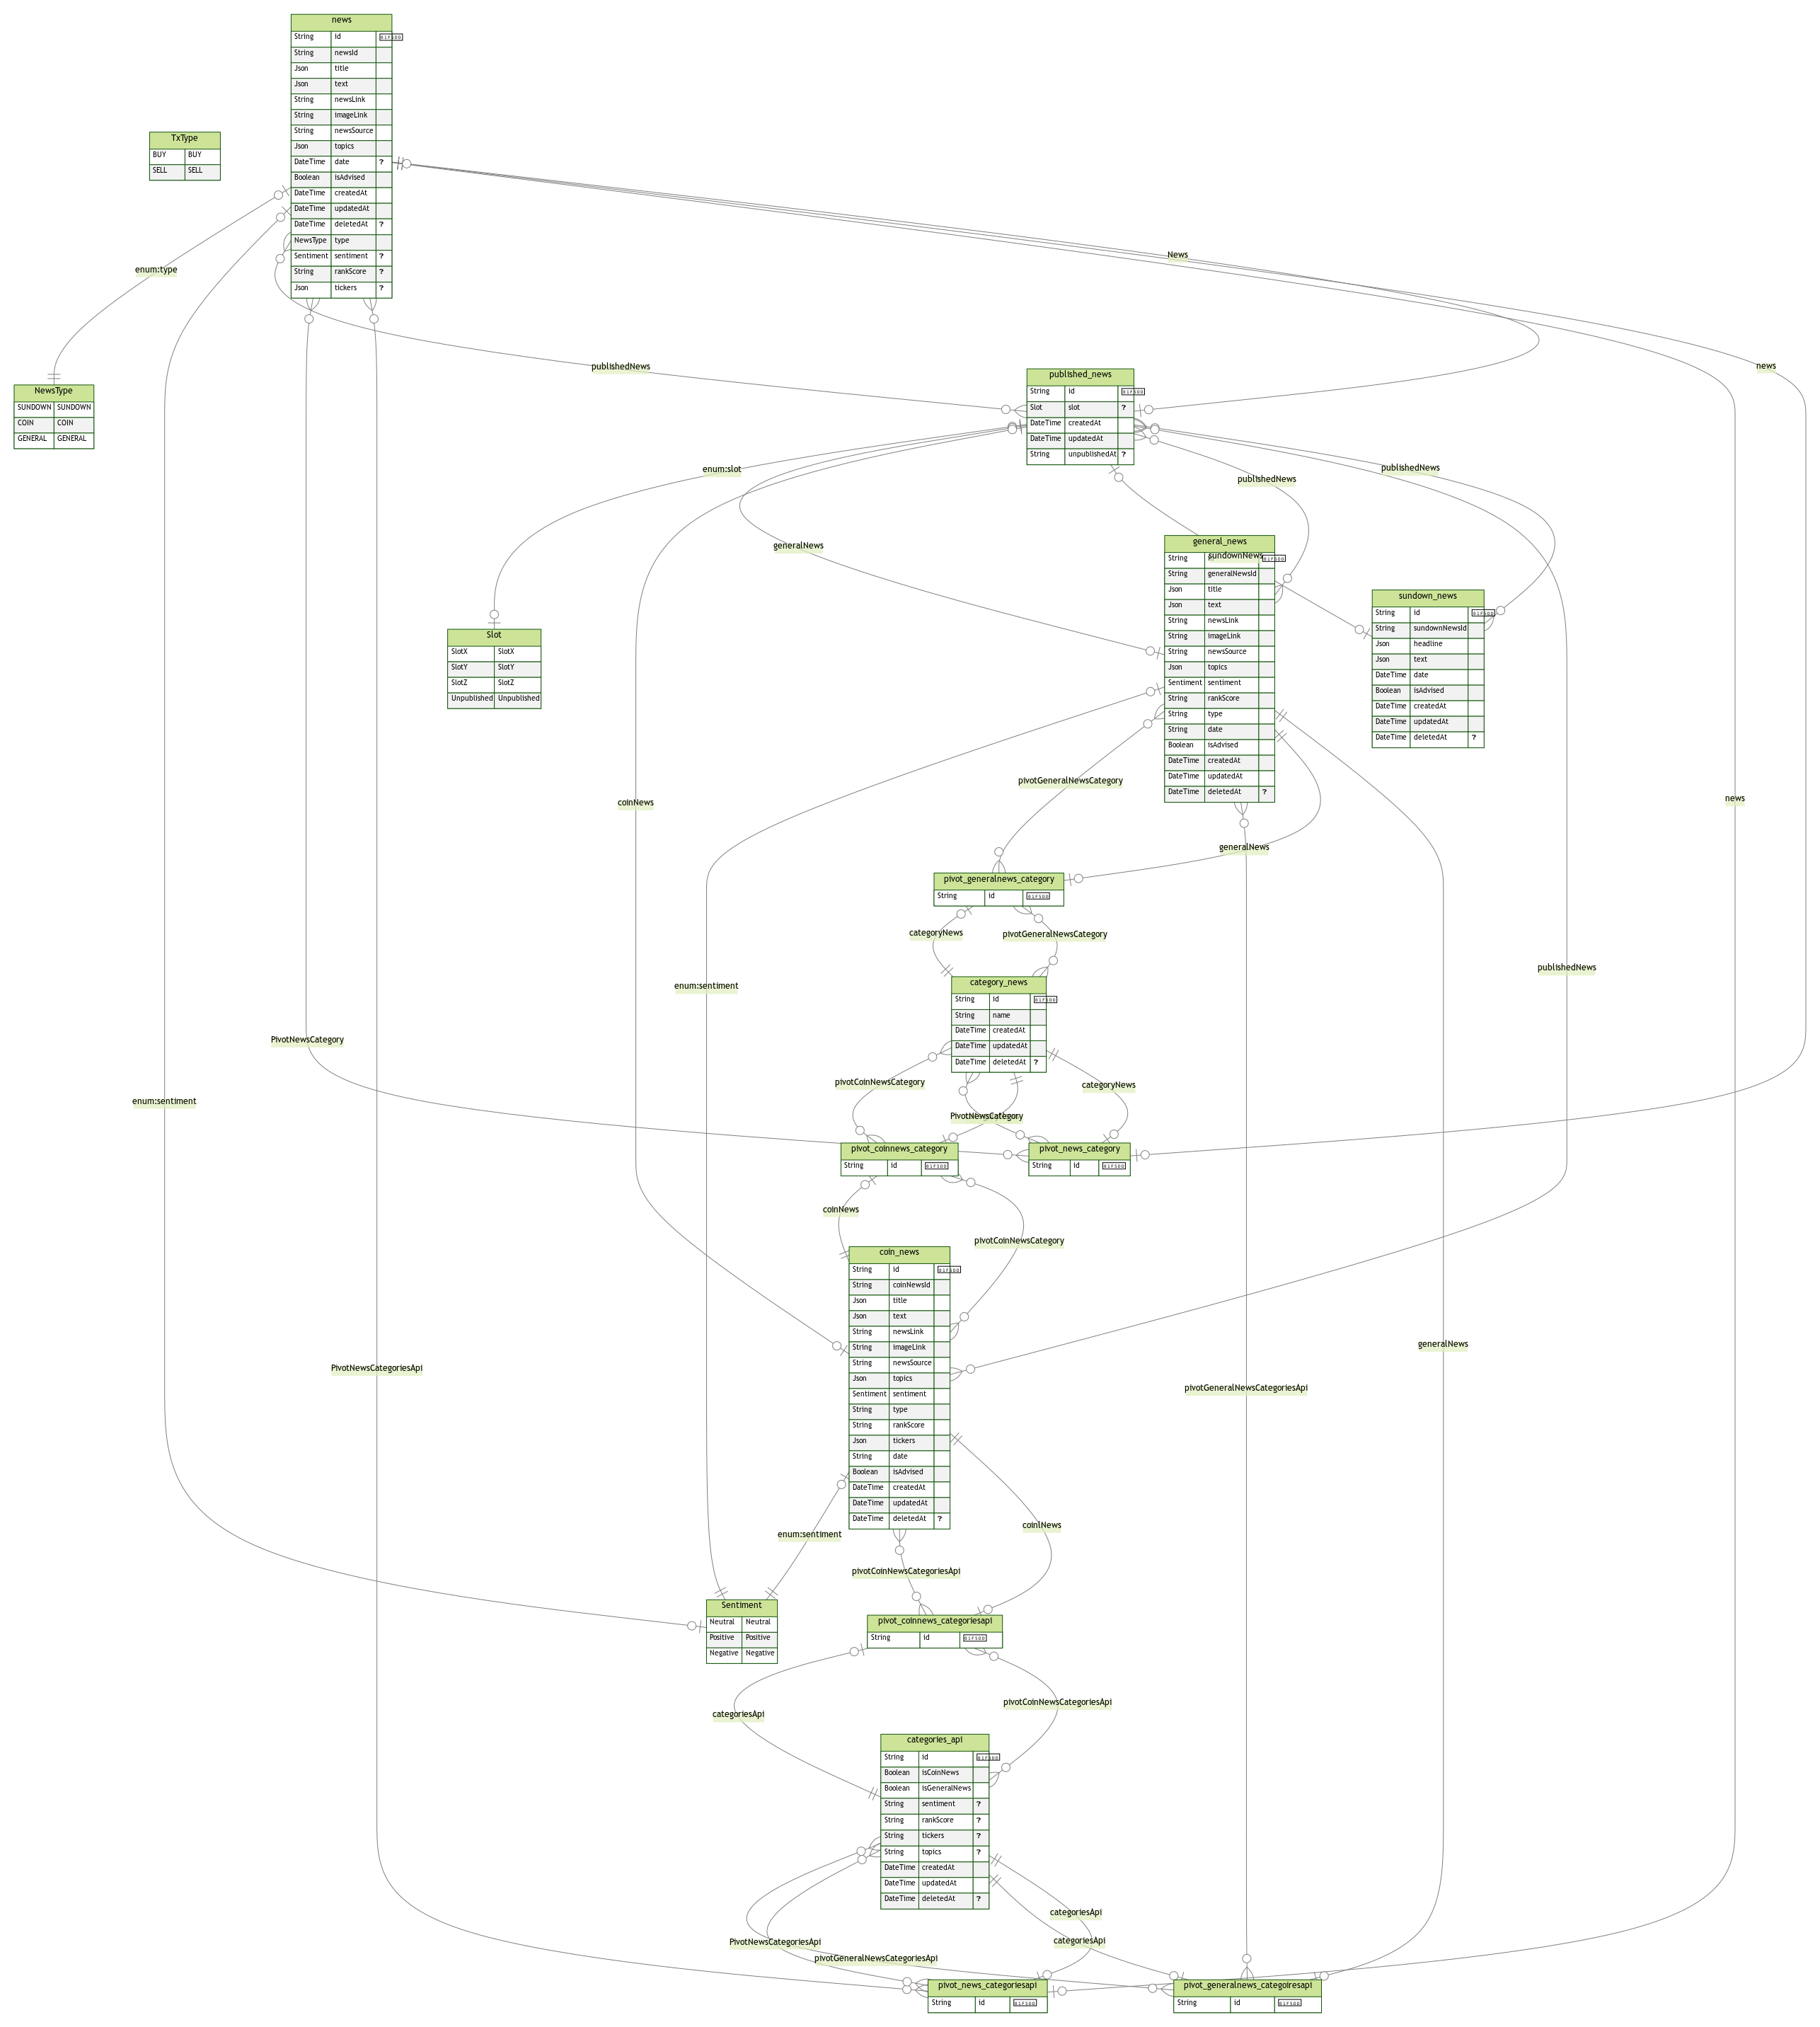
\includegraphics[width=\textwidth,height=\textheight,keepaspectratio]{ERD.png} % Adjusts the size to fit the page
\caption{Entity Relationship Diagram of the System} % Optional: add a caption
\label{fig:er_diagram} % Optional: label for referencing the figure
\end{figure}
\clearpage % Ensures any following content appears on a new page

\clearpage % Ensures the image appears on a new page
\begin{figure}[p] % 'p' places the figure on a page containing only floats, such as tables and figures.
\centering % Centers the image
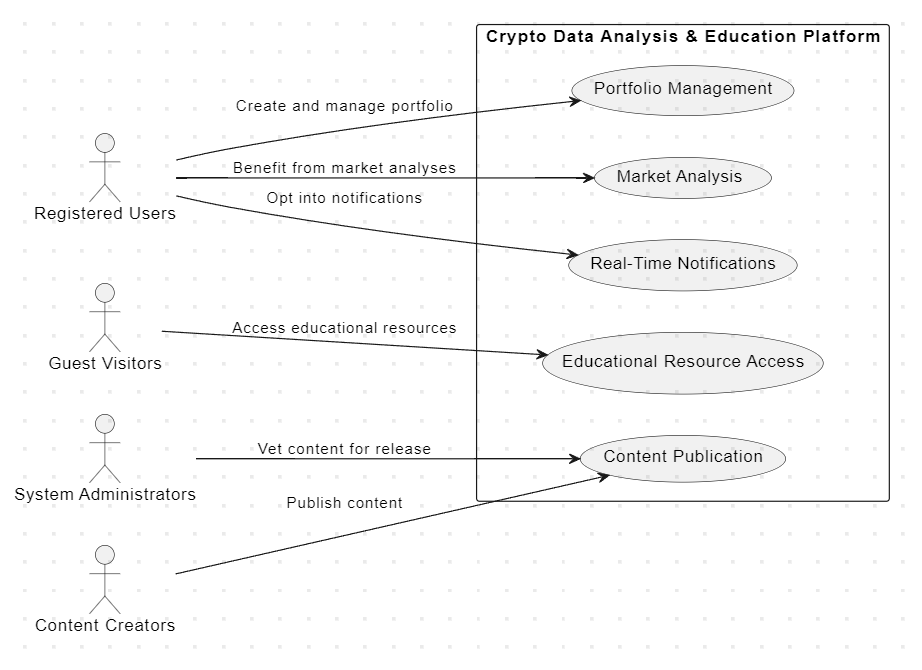
\includegraphics[width=\textwidth,height=\textheight,keepaspectratio]{use-case.png} % Adjusts the size to fit the page
\caption{Use Case Diagram of the System} % Optional: add a caption
\label{fig:er_diagram} % Optional: label for referencing the figure
\end{figure}
\clearpage % Ensures any following content appears on a new page

\begin{thebibliography}{9}
\bibitem{nakamoto2008}
Nakamoto, S. (2008). \textit{Bitcoin: A peer-to-peer electronic cash system}. Retrieved from \url{https://bitcoin.org/bitcoin.pdf}

\bibitem{antonopoulos2017}
Antonopoulos, A. M. (2017). \textit{Mastering Bitcoin: Programming the open blockchain}. O'Reilly Media, Inc.

\bibitem{buterin2014}
Buterin, V. (2014). \textit{A next-generation smart contract and decentralized application platform}. Retrieved from \url{https://ethereum.org/en/whitepaper/}

\bibitem{drescher2017}
Drescher, D. (2017). \textit{Blockchain basics: A non-technical introduction in 25 steps}. Apress.

\bibitem{zheng2018}
Zheng, Z., Xie, S., Dai, H. N., Chen, X., \& Wang, H. (2018). Blockchain challenges and opportunities: A survey. \textit{International Journal of Web and Grid Services}, 14(4), 352-375.

\bibitem{mougayar2016}
Mougayar, W. (2016). \textit{The business blockchain: Promise, practice, and application of the next Internet technology}. John Wiley \& Sons.

\bibitem{tapscott2016}
Tapscott, D., \& Tapscott, A. (2016). \textit{Blockchain revolution: How the technology behind bitcoin is changing money, business, and the world}. Penguin.

\bibitem{swan2015}
Swan, M. (2015). \textit{Blockchain: Blueprint for a new economy}. O'Reilly Media, Inc.


\bibitem{kose2022}
Köse, C. (2022). \textit{Title of the article or book chapter on cryptocurrency education platforms}. 

\end{thebibliography}




\section{Choose Interdisciplinary Domain of Study}
[8.Decent Work and Economic Growth]

\end{document}
